\section{Administración de archivos de configuración}
La administración de archivos de configuración se divide en dos partes. La importación y la exportación. Para ambos casos se utilizó FTP como protocolo de intercambio de archivos. Ambas funciones se encuentran definidas dentro del programa \textbf{cliente.py} y cada una de ellas necesita un archivo de configuración en el que se definen las direcciones IP destino u origen, rutas de archivos, usuarios y contraseñas, etc.

\subsubsection{Importación}
El archivo de configuración para la función de importación se puede observar en la figura \ref{image:import-conf}. Podemos observar que en la parte superior se define la sintaxis de cada regla. Esto permite agregar los parámetros de diferentes routers y que la ejecución del programa sea fluido.

\FloatBarrier
\begin{figure}[htbp!]
		\centering
			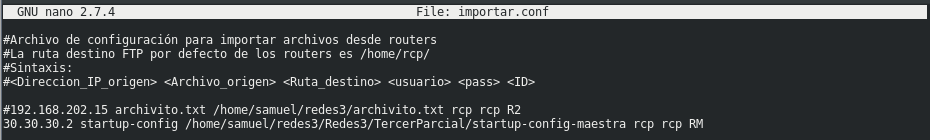
\includegraphics[width=.55 \textwidth]{images/import-conf}
		\caption{Archivo de configuracion para importaciones.}
		\label{image:import-conf}
\end{figure}
\FloatBarrier

El código de la función \textbf{importar()} se puede ver en la figura \ref{image:import-codigo}. Que consiste básicamente en un ciclo que busca líneas que no comiencen con el caracter \#, es decir, que no estén comentadas. Una vez que obtiene una línea descompone la cadena y obtiene los parámetros necesarios para realizar una conexión FTP y la respectiva descarga del archivo (también definido en el archivo de configuración). 

\FloatBarrier
\begin{figure}[htbp!]
		\centering
			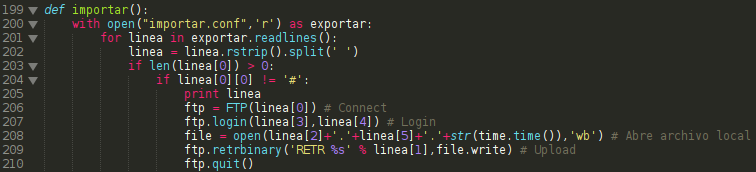
\includegraphics[width=.55 \textwidth]{images/import-codigo}
		\caption{Código para importar archivos.}
		\label{image:import-codigo}
\end{figure}
\FloatBarrier

El funcionamiento se puede observar en la figura \ref{image:import-func}.

\FloatBarrier
\begin{figure}[htbp!]
		\centering
			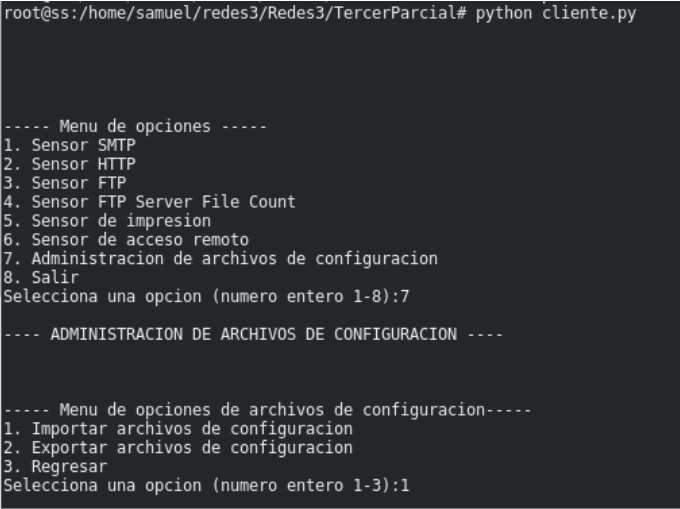
\includegraphics[width=.55 \textwidth]{images/import-func}
		\caption{Funcionamiento de la importación de archivos.}
		\label{image:import-func}
\end{figure}
\FloatBarrier

\subsubsection{Exportación}
El archivo de configuración para la función de exportación se puede observar en la figura \ref{image:export-conf}. Podemos observar que en la parte superior se define la sintaxis de cada regla. Al igual que la importación, esto permite agregar los parámetros de diferentes routers y que la ejecución del programa sea fluido.

\FloatBarrier
\begin{figure}[htbp!]
		\centering
			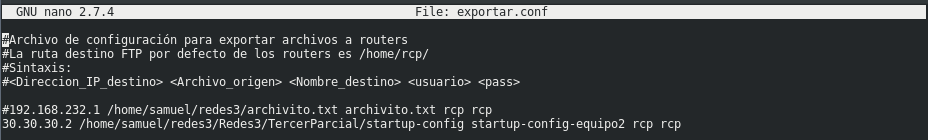
\includegraphics[width=.55 \textwidth]{images/export-conf}
		\caption{Archivo de configuracion para exportaciones.}
		\label{image:export-conf}
\end{figure}
\FloatBarrier

El código de la función \textbf{exportar()} se puede ver en la figura \ref{image:export-codigo}. Que, al igual que \textbf{importar()}, consiste básicamente en un ciclo que busca líneas que no comiencen con el caracter \#, es decir, que no estén comentadas. Una vez que obtiene una línea descompone la cadena y obtiene los parámetros necesarios para realizar una conexión FTP y la respectiva subida del archivo (también definido en el archivo de configuración). 

\FloatBarrier
\begin{figure}[htbp!]
		\centering
			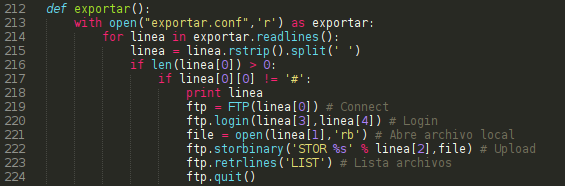
\includegraphics[width=.55 \textwidth]{images/export-codigo}
		\caption{Código para exportar archivos.}
		\label{image:export-codigo}
\end{figure}
\FloatBarrier

El funcionamiento se puede observar en la figura \ref{image:export-func}.

\FloatBarrier
\begin{figure}[htbp!]
		\centering
			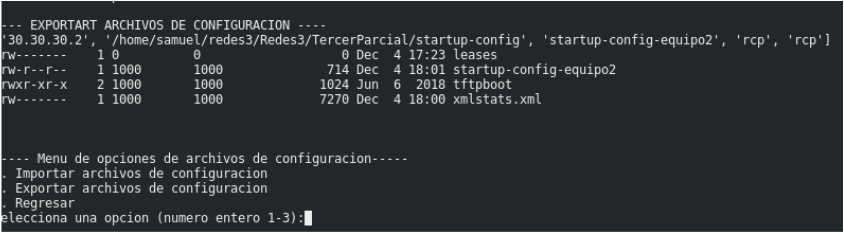
\includegraphics[width=.55 \textwidth]{images/export-func}
		\caption{Funcionamiento de la exportación de archivos.}
		\label{image:export-func}
\end{figure}
\FloatBarrier